\chapter{Resposta em Sala de Aula}

As principais tecnologias, ferramentas e métodos foram descritos nos capítulos
anteriores. Como resultado final foi desenvolvido um sistema de resposta
em sala de aula denominado \textit{Resposta em Sala de Aula}.

\section{Aplicação web para o Professor}

A \autoref{fig:main_window} ilustra a tela inicial da aplicação web para o professor.
Nela é possível perceber as três abas principais do sistema. A primeira \textit{Questões} que
está selecionada, permite ao professor gerir um banco de questões criadas, iniciar uma
sessão com questões selecionadas e categorizar as questões para uma melhor organização das mesmas.

\begin{figure}[ht]
  \centering
  \caption{Aba \textit{Questões}}
  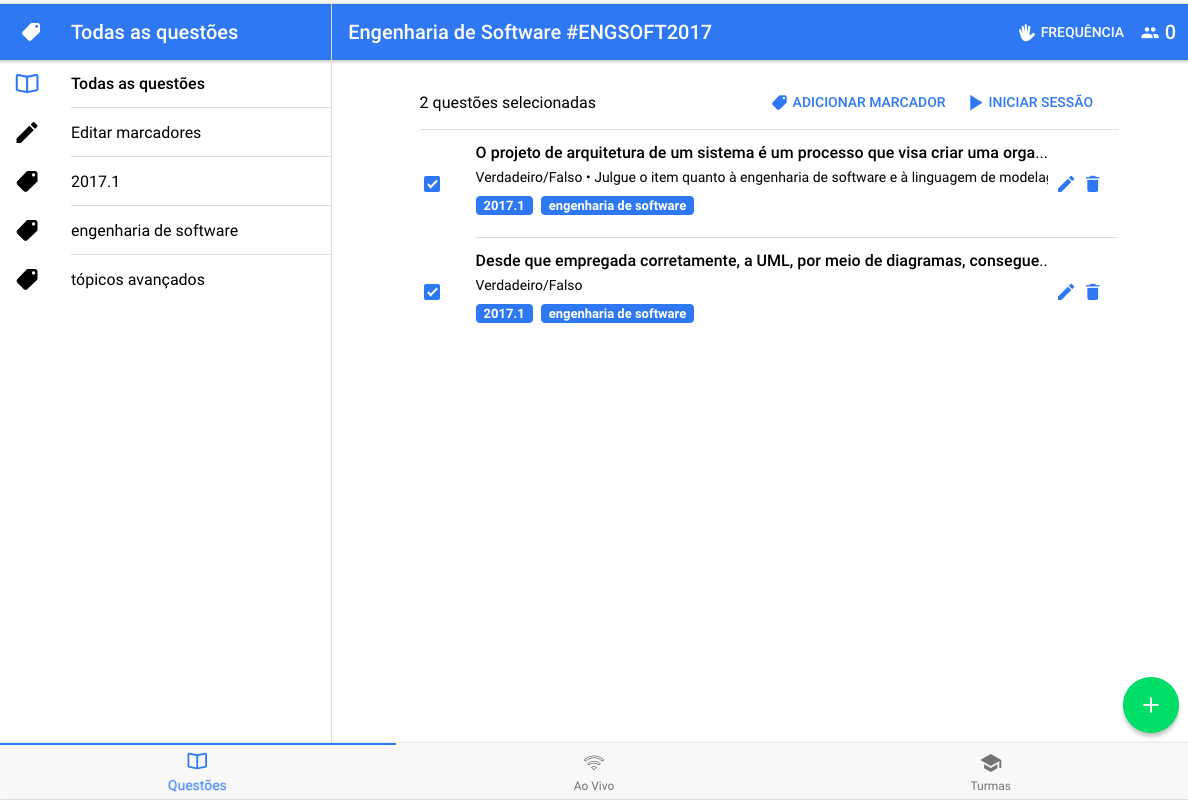
\includegraphics[scale=.40]{imagens/telas/main_window}
  \doautor
  \label{fig:main_window}
\end{figure}

\subsection{Frequência dos alunos}
\label{sec:freq_students}

Um dos requisitos do sistema era permitir ao professor realizar a frequência dos alunos
pelo aplicativo. O sistema gera um código aleatório de quatro digitos e permite aos estudantes
submeterem esse código pelo aplicativo. O professor pode ativar a frequência
clicando no botão \textit{Frequência} no canto superior direito da aba \textit{Questões} (\autoref{fig:main_window}).
Em seguida, o sistema muda para a aba \textit{Ao Vivo}, tendo como resultado a \autoref{fig:live_freq}.
Nela é possível perceber o código de aleatório de quatro dígitos que foi gerado e alguns botões de ação no canto
inferior direto, permitindo ao professor encerrar a frequência por exemplo.

\begin{figure}[ht]
  \centering
  \caption{Página para a realizar a frequência dos estudantes}
  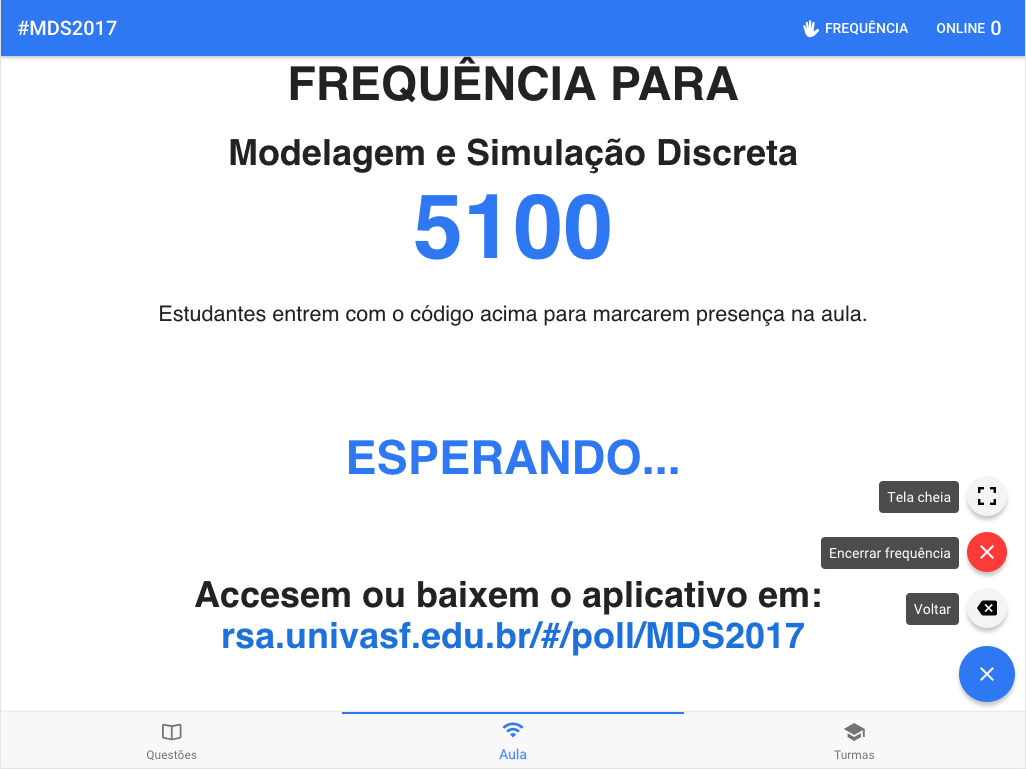
\includegraphics[scale=.45]{imagens/telas/live_freq}
  \doautor
  \label{fig:live_freq}
\end{figure}

Posteriormente, o professor pode acessar a lista de frequência por meio do aba \textit{Turmas},
clicando para cada turma a opção de \textit{atividades}, \autoref{fig:atividades}. A \autoref{fig:list_freq} exibe a
lista de frequência em detalhes.

\begin{figure}[ht]
  \centering
  \caption{Página para a realizar a frequência dos estudantes}
  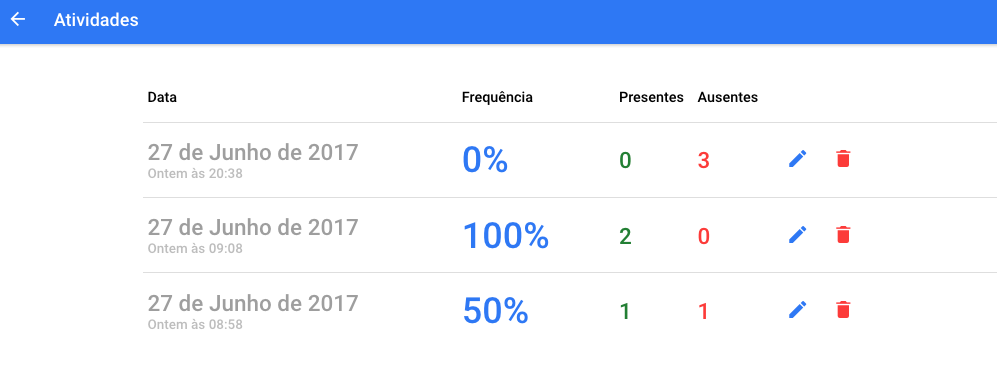
\includegraphics[scale=.45]{imagens/telas/atividades}
  \doautor
  \label{fig:atividades}
\end{figure}

\begin{figure}[ht]
  \centering
  \caption{Página para a realizar a frequência dos estudantes}
  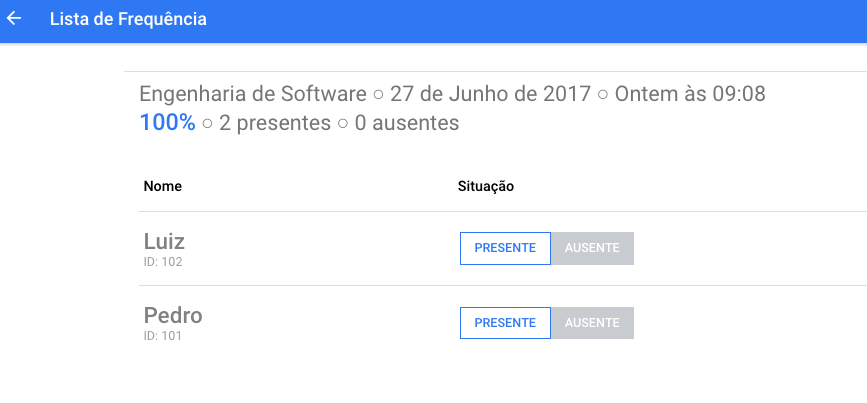
\includegraphics[scale=.45]{imagens/telas/list_freq}
  \doautor
  \label{fig:list_freq}
\end{figure}


\subsection{Cadastro de Questões}

A \autoref{fig:new_question} exibe o formulário para o cadastro de uma nova questão.
A aplicação permite a criação de questões de múltipla escolha, verdadeiro e falso e questão aberta.
Em questões do tipo múltipla escolha o professor deve indicar uma alternativa como correta.

\begin{figure}[ht]
  \centering
  \caption{Formulário \textit{Nova Questão}}
  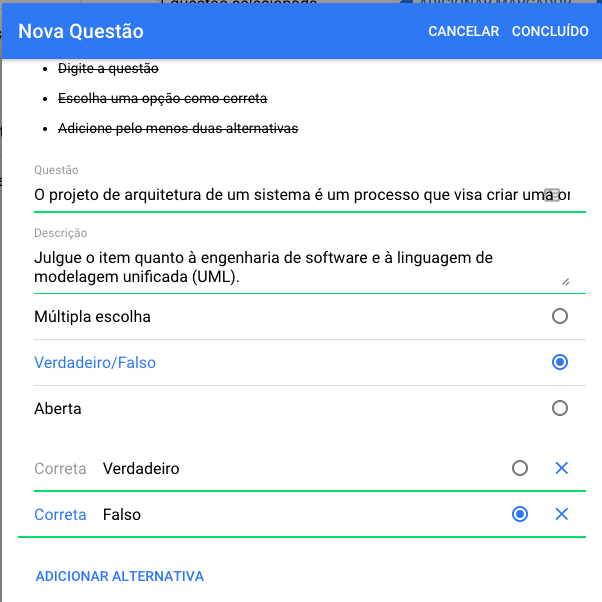
\includegraphics[scale=.5]{imagens/telas/new_question}
  \doautor
  \label{fig:new_question}
\end{figure}

\subsection{Turmas}
\label{subsection:turmas}

Na aba de \textit{Turmas} (\autoref{fig:admin_classes}), o professor faz o cadastro das turmas
para permitir acesso aos estudantes. Foi criado o conceito de \textit{turmas públicas}
e \textit{turmas privadas}. Uma turma pública é aquele em que não existe uma
lista de alunos cadastrados, ou seja, qualquer aluno com o código de acesso da turma
vai poder acessar e participar das atividades apenas digitando o código de acesso.

Quando uma lista de estudantes é adicionada em uma turma (a \autoref{fig:add_students} ilustre esse processo) ela se
torna uma turma privada. Quando os estudantes acessarem a turma eles terão que
digitar além do código da turma, o código de identificação de cada um que foi cadastrado no sistema.

\begin{figure}[ht]
  \centering
  \caption{Aba \textit{Turmas}}
  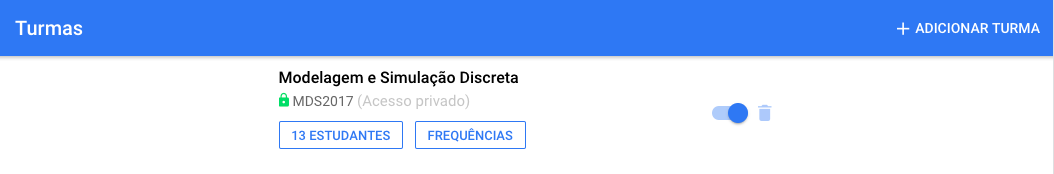
\includegraphics[scale=.4]{imagens/telas/admin_classes}
  \doautor
  \label{fig:admin_classes}
\end{figure}

\subsubsection{Lista de estudantes em uma turma}

A \autoref{fig:add_students} ilustra o cadastro de estudantes de uma turma.
O professor tem a opção de adicionar manualmente cada estudante, clicando
na opção \textit{Adicionar manualemente} no canto inferior direito, digitando
o nome do estudante e o código de identificação (esse é o código que os estudantes
terão que digitar além do código da sala para ter acesso).

A outra opção para adicionar a lista de estudantes é importar um arquivo CSV
contendo o nome dos estudantes e código de identificação, clicando
na opção \textit{Importar Estudantes (CSV)} no canto inferior direito. Um exemplo de um
arquivo CSV válido para importação é ilustrado na \autoref{fig:import_csv}.
A importação do arquivo CSV trata a primeira linha como o cabelçalho de coluna,
e deve conter exclusivamente \texttt{name,id}. Nas outras linhas deve incluir
primeiro o nome do estudante e depois o código de identificação.

\begin{figure}[ht]
  \centering
  \caption{Adicionar estudantes em uma turma}
  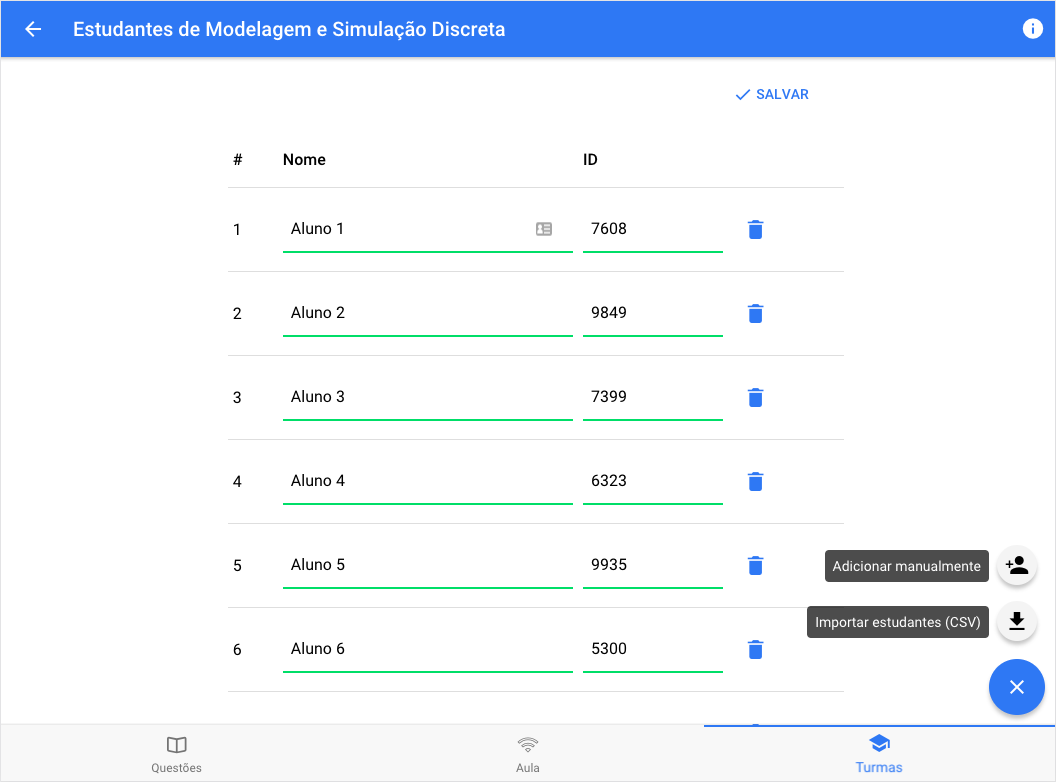
\includegraphics[scale=.4]{imagens/telas/add_students}
  \doautor
  \label{fig:add_students}
\end{figure}

\begin{figure}[ht]
\caption{Exemplo de arquivo CSV válido para importar uma lista de estudantes}
\begin{lstlisting}[language=JavaScript]
  name,id
  Alexandre Gabriel Daniel Freitas,42160120863
  Lucas Elias Antonio Mendes,83562725728
  Igor Isaac Alves,24356903986
  Diego Marcelo Leonardo Ribeiro,87528468061
  Marcos Vinicius Diego da Silva,69525285553
  Arthur Ryan Barbosa,45863716258
  Elias Raul Calebe Cardoso,17505265300
  Paulo Thiago Costa,55883747540
  Carlos Eduardo Henry Cardoso,24051360318
  Ricardo Giovanni Bryan Pereira,84740254433
  Helena Ester Rayssa Costa,84617846859
  Maria Bruna Cardoso,45713856925
  Stefany Mariana Sophie Pereira,65113718408
  Isabel Nina Gomes,16108646020
\end{lstlisting}
  \doautor
\label{fig:import_csv}
\end{figure}

\subsection{Sessão de questões: Aba Ao Vivo}

No sistema tem-se o conceito de \textit{Sessão de questões}, que é
simplesmente um conjunto de questões selecionadas pelo professor
para apresentar para os estudantes.

O professor pode iniciar uma sessão na aba \textit{Questões}, selecionando
uma ou mais questões que deseja apresentar para os estudantes e
em seguida clicar no botão \textit{INICIAR SESSÃO}. A \autoref{fig:session_details}
destaca da aba \textit{Questões} um exemplo de duas questões selecionadas e o botão
\textit{INICIAR SESSÃO} no canto superior direto. Quando o professor inicia uma sessão,
o sistema redireciona para a aba \textit{Ao Vivo} projetando a primeira questão selecionada (\autoref{fig:live})

\begin{figure}[ht]
  \centering
  \caption{Aba \textit{Questões}}
  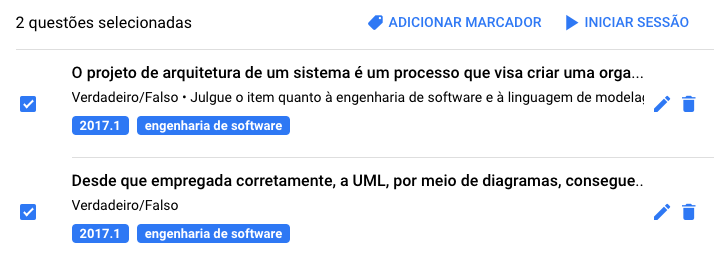
\includegraphics[scale=.50]{imagens/telas/session_details}
  \doautor
  \label{fig:session_details}
\end{figure}

A \autoref{fig:live} ilustra uma sessão iniciada de uma questão. Uma questão quando
iniciada ainda não fica disponível para os estudantes responderem, que está indicado
na parte superior da tela com o texto \textit{VOTAÇÃO INDISPONÍVEL}. Nessa mesma parte,
o código para acesso da sala fica visível para os estudantes, no caso \textit{ENGSOFT2017}.

No canto inferior direito da \autoref{fig:live}, o professor tem acesso a um conjunto de
funcionalidades para controlar a sessão. A opção \textit{Ativar votação}, quando selecionada
permite ao professor disponibilizar para os alunos a questão que está sendo exibida para que
eles possam responder no aplicativo (a \autoref{subsecao:alunosrespondem} detalha esse processo).
As opções \textit{Mostrar resposta} e \textit{Mostrar resultado} permitem respectivamente indicar
na tela a alternativa correta e exibir na tela como os estudantes responderam.
No canto superior direito da tela um número é incrementado indicando a quantidade de
alunos que já responderam a questão. A \autoref{fig:live_answers} ilustra quando
todas essas opções estão selecionadas.

\begin{figure}[ht]
  \centering
  \caption{Adicionar estudantes em uma turma}
  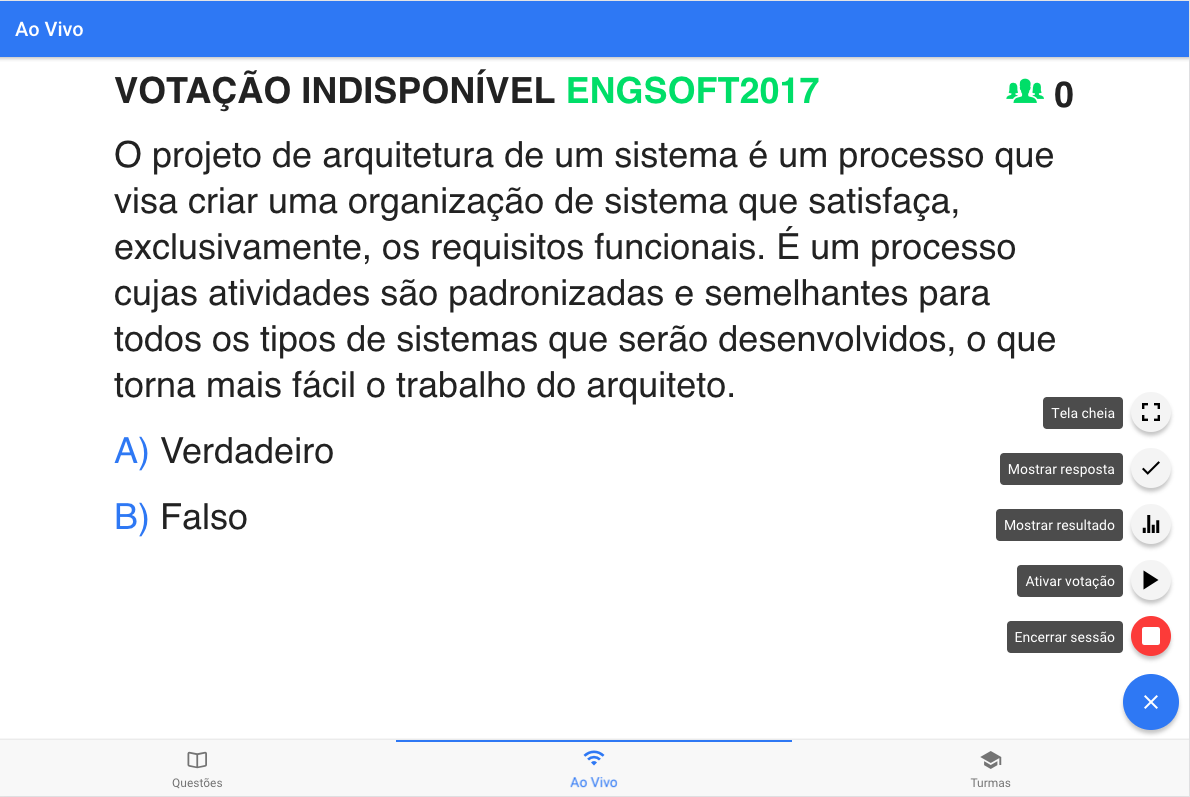
\includegraphics[scale=.4]{imagens/telas/live}
  \doautor
  \label{fig:live}
\end{figure}

\begin{figure}[ht]
  \centering
  \caption{Adicionar estudantes em uma turma}
  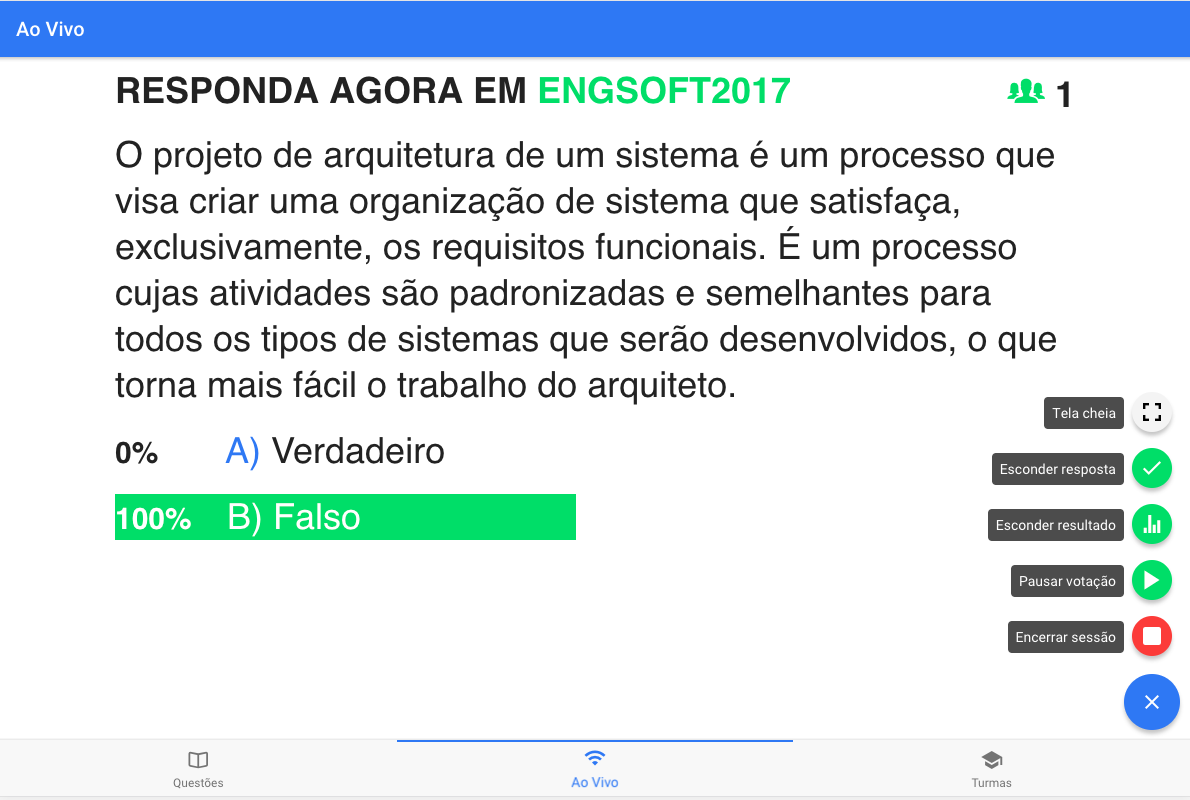
\includegraphics[scale=.4]{imagens/telas/live_answers}
  \doautor
  \label{fig:live_answers}
\end{figure}

\subsubsection{Sessões encerradas}

Quando uma sessão é encerrada, clicando no botão \textit{Encerrar sessão} no canto inferior direito
exibido na \autoref{fig:live}, uma lista das sessões encerradas é mostrado, indicando
o nome da turma, a quantidade de questões, o número de alunos participantes e a data da sessão, como
exibido na \autoref{fig:sessions}.

Clicando em um item dessa lista, é possível ver como cada estudante respondeu as questões e um
desempenho geral da turma por questão. A \autoref{fig:session_students_details}  exibe o
desempenho de cada estudante por questão e a percentagem de acerto na sessão.

\begin{figure}[ht]
  \centering
  \caption{Adicionar estudantes em uma turma}
  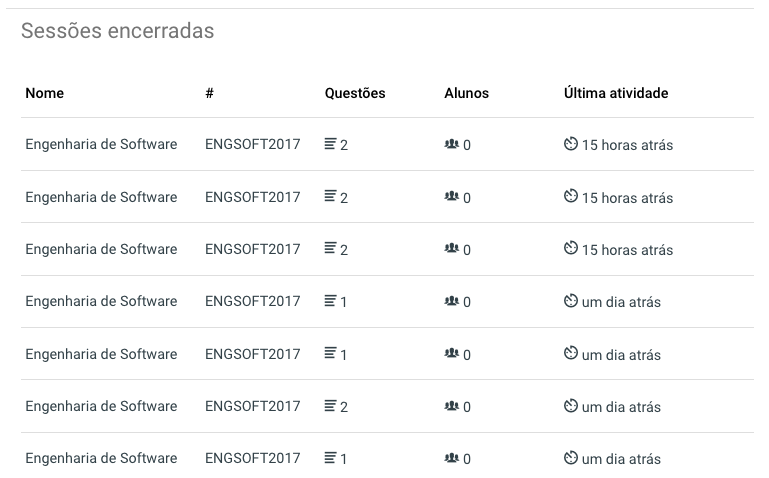
\includegraphics[scale=.4]{imagens/telas/sessions}
  \doautor
  \label{fig:sessions}
\end{figure}

\begin{figure}[ht]
  \centering
  \caption{Adicionar estudantes em uma turma}
  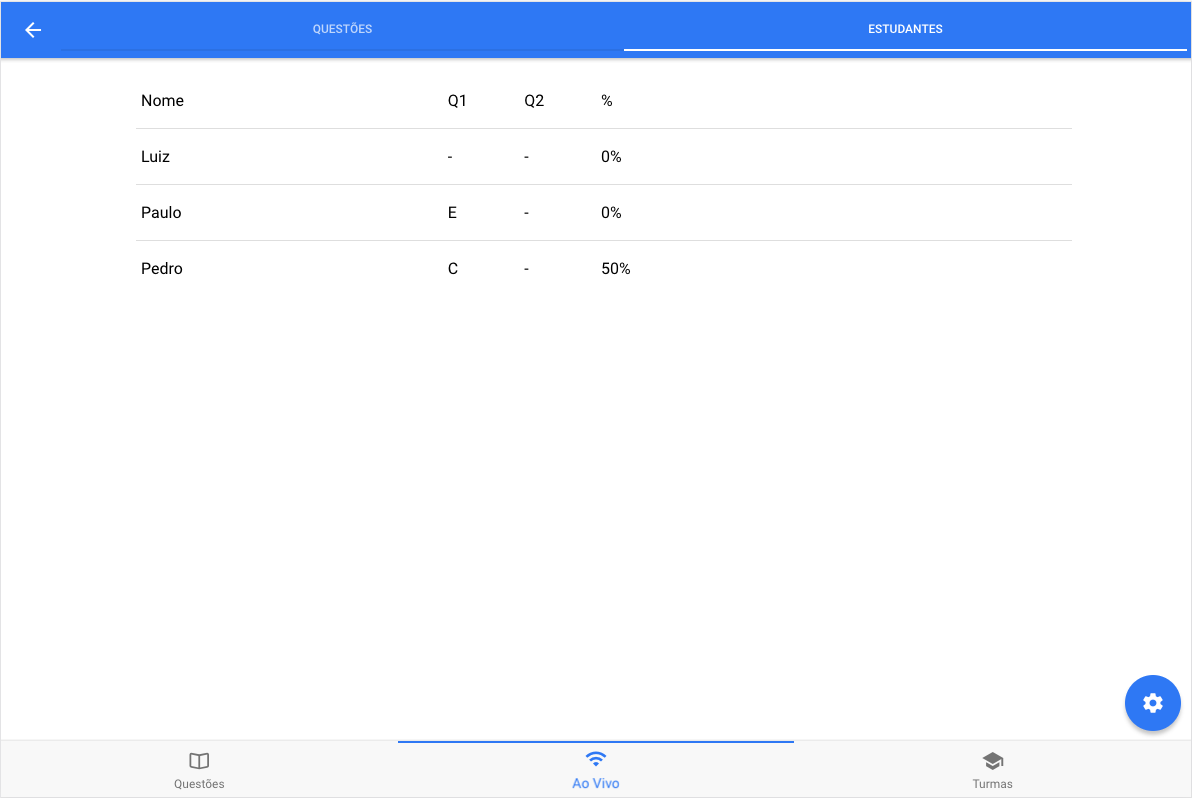
\includegraphics[scale=.4]{imagens/telas/session_students_details}
  \doautor
  \label{fig:session_students_details}
\end{figure}

\clearpage

\section{Aplicação para dispositivos móveis, que será utilizado como {\clickers}}

A \autoref{fig:app_home} exibe a tela inicial do aplicativo em que é possível perceber
um campo para que os estudantes possam digitar o código de acesso da turma, conforme detalhou-se
na \autoref{subsection:turmas}.

\begin{figure}[ht]
  \centering

  \caption{Tela inicial da aplicação móvel do estudante}

  \subfloat[Campo indicando para digitar o código de acesso]{
    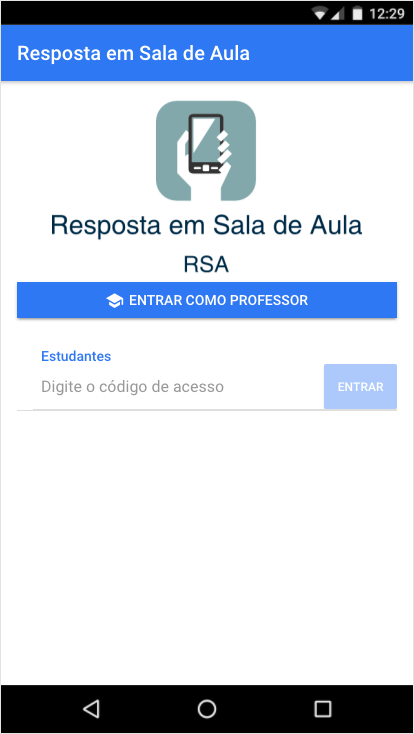
\includegraphics[scale=.4]{imagens/telas/app_home_sem}
  }$\quad$
  \subfloat[Exemplo de código de acesso digitado] {
    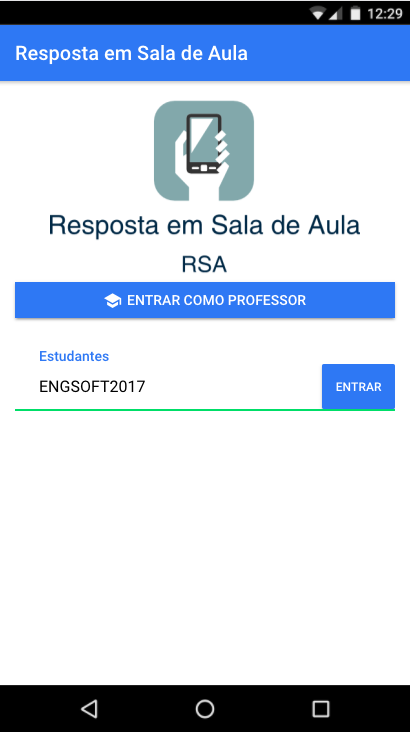
\includegraphics[scale=.4]{imagens/telas/app_home}
  }

  \doautor
  \label{fig:app_home}
\end{figure}


\subsection{Identificação dos estudantes}

Conforme apresentado na \autoref{subsection:turmas} tem-se o conceito
de turmas públicas (que permitem acesso a turma apenas com o código da turma) e
as turmas privadas que além do código da turma é necessário o código de identificação
do estudante cadastrado previamente pelo professor.

A \autoref{fig:app_ask_id} ilustra o processo de identificação do estudante
considerando que o acesso a turma é privado. Na \autoref{fig:app_ask_a} o aplicativo
exibe uma mensagem e um campo para que o estudante digite o código de
identificação único do estudante. A \autoref{fig:app_ask_b}, exibe a tela
quando o estudante digita o código correto, detalhando o nome do estudante, do professor e da turma.

\begin{figure}[ht]
  \centering

  \caption{Tela de identificação dos estudantes}

  \subfloat[Código de identificação]{
    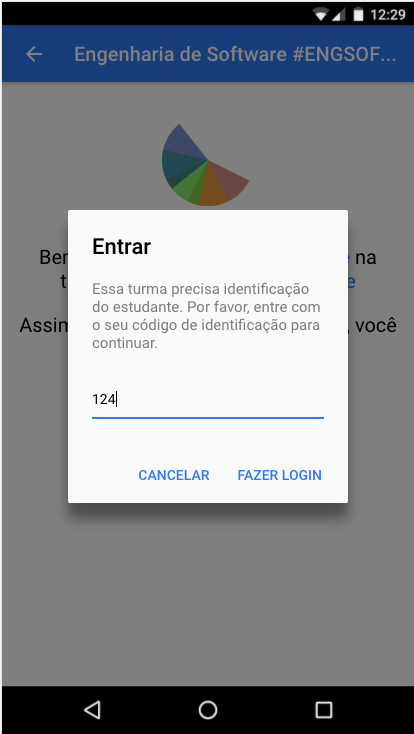
\includegraphics[scale=.4]{imagens/telas/app_ask_id}
    \label{fig:app_ask_a}
  }$\quad$
  \subfloat[Detalhes do estudante, professor e da turma] {
    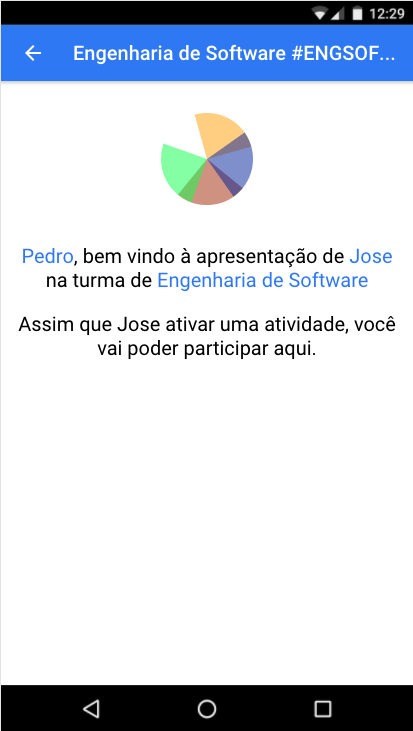
\includegraphics[scale=.4]{imagens/telas/app_ask_success}
    \label{fig:app_ask_b}
  }

  \doautor
  \label{fig:app_ask_id}
\end{figure}

\subsection{Responder frequência}

Na \autoref{sec:freq_students} tem-se o processo para o professor realizar
a frequência dos estudantes. Quando o professor habilita para os
estudantes enviarem o código de quatro dígitios gerado, um botão aparece
no aplicativo dos estudantes com a opção \textit{Responder chamada} no canto inferior
direito, como mostra na \autoref{fig:freqa}. Em seguida, quando o estudante
clica nesse botão, o aplicativo exibe uma mensagem e um campo para que os
estudantes digitem o código disponibilizado pelo professor (\autoref{fig:freqb}).

\begin{figure}[ht]
  \centering

  \caption{Telas para os estudantes realizarem a frequência}

  \subfloat[Botão para responder a chamada]{
    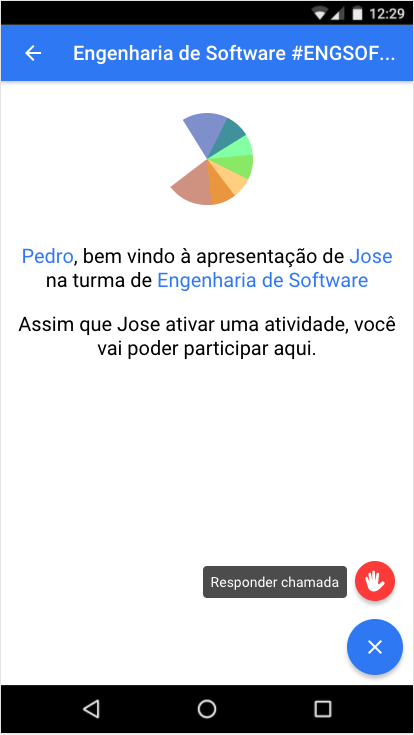
\includegraphics[scale=.35]{imagens/telas/student_freq1}
    \label{fig:freqa}
  }$\quad$
  \subfloat[Tela com campo para digitar código] {
    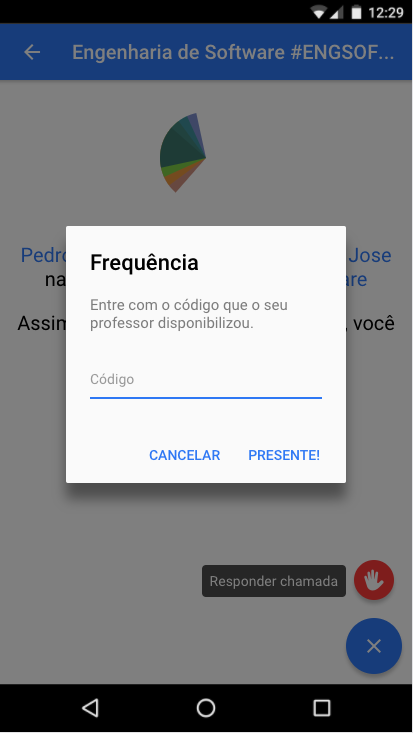
\includegraphics[scale=.35]{imagens/telas/student_freq2}
    \label{fig:freqb}
  }
  \label{fig:freqalunos}

  \doautor
\end{figure}


\subsection{Responder questões}\label{subsecao:alunosrespondem}

O sistema permite ao professor criar questões de múltipla escolha e
de resposta livre. A \autoref{fig:student_q} ilustra como fica
apresentado no aplicativo as questões. A \autoref{fig:student_qa} exibe
uma questão de verdadeiro e falso e a \autoref{fig:student_qb} ilustra
uma questão aberta.

\begin{figure}[ht]
  \centering
  \caption{Diferentes tipos de questões no aplicativo}

  \subfloat[Questão do tipo múltipla escolha]{
    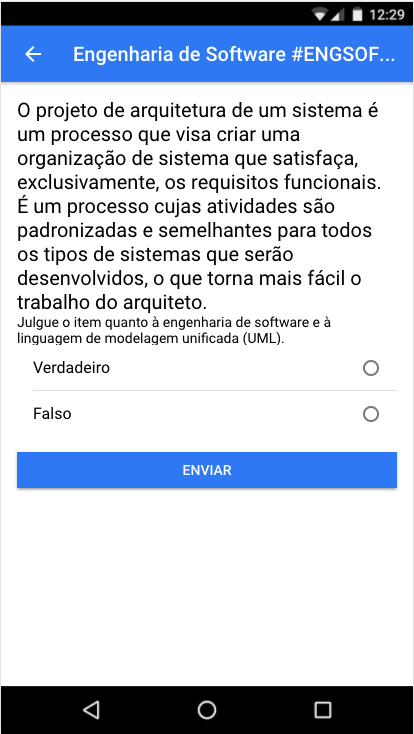
\includegraphics[scale=.35]{imagens/telas/student_question1}
    \label{fig:student_qa}
  }$\quad$
  \subfloat[Questão do tipo resposta curta] {
    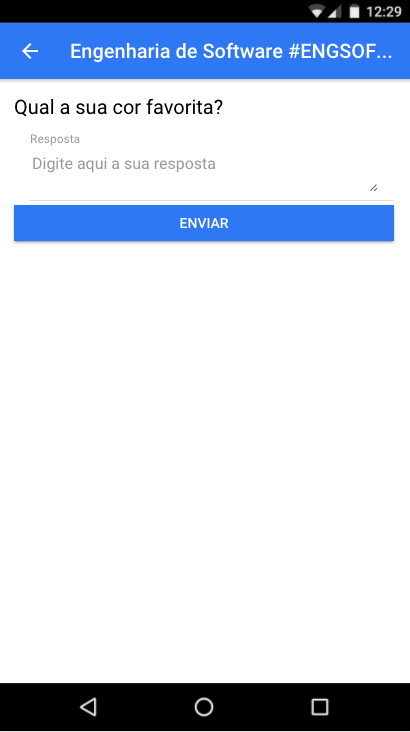
\includegraphics[scale=.35]{imagens/telas/student_question2}
    \label{fig:student_qb}
  }

  \doautor
    \label{fig:student_q}
\end{figure}
